%!TEX root = linear-algebra.tex
\stepcounter{lecture}
\setcounter{lecture}{1}
\pagebreak
\sektion{Kinematics}
\setcounter{page}{4}

What \lecturemarker{1}{5 Oct} we are after is an \emph{equation of motion} to find the position of an object for all times. Ingredients to an equation of motion:\begin{enumerate}
\item[1)] Kinematics - Description of motion 
\item[2)] Kinetics - Newton's laws
\item[3)] Mathematical Description of Forces - Describe forces in terms of kinematic quantities
\end{enumerate}


\subsektion{Cartesian Coordinates} % (fold)
\label{sub:sets}



For a point particle there are three key kinematic quantities.\begin{enumerate}
\item[1.] Positon: $\vec{r}(t)$
\item[2.] Velocity: $\vec{v}(t)$
\item[3.] Acceleration: $\vec{a}(t)$

In general, $\vec{r}(t),~\vec{v}(t),~\vec{a}(t) \in \mathbb{R}^3$. 
\end{enumerate}\vspace*{5pt}

We can use different coordinate systems to describe our quantities:
\begin{enumerate}
\item Cartesian
\item Polar
\item Intrinsic	
\end{enumerate}

Consider the path of a particle through space:

\vspace*{100pt}

\begin{definition} We write the \emph{position} at time $t$ as
\[\vec{r}(t) = x(t)\hat{i} + y(t)\hat{j} + z(t)\hat{k}\]
We can also write this as
\[[\vec{r}(t)] = \left[\begin{smallmatrix}
x(t)\\ y(t) \\ z(t)	
\end{smallmatrix}
 \right]\text{ so, } \hat{i} =  \left[\begin{smallmatrix}
1\\0\\0
\end{smallmatrix}
 \right],~ \hat{j} =  \left[\begin{smallmatrix}
0\\j\\0
\end{smallmatrix}
 \right],~ \hat{k} =  \left[\begin{smallmatrix}
0\\0\\1
\end{smallmatrix}
 \right]\]
 \textit{Magnitude of $\vec{r}$} \[r = |\vec{r}| = \sqrt{x^2 + y^2 + z^2}\]
$r$ is the distance from the origin.
 
 \textit{Direction of $\vec{r}$} \[\hat{r} = \vec{r}/r = \frac{x}{r}\hat{i} + \frac{y}{r}\hat{j} + \frac{z}{r}\hat{k}\]
  \end{definition}
  
 So, we can write 
 \[\vec{r} = r(t)\hat{r}(t)\]
 This is the starting point for polar coordinates.\\

  \lecturemarker{2}{5 Oct}
 \textbf{Last Time:}
 \vspace*{100pt}



Position: 
\[\vec{r}(t) = x(t)\hat{i} + y(t)\hat{j} + z(t)\hat{k}\]
At $\Delta t$ later
\[\vec{r}(t + \Delta t) = x(t + \Delta t)\hat{i} + y(t + \Delta t)\hat{j} + z(t + \Delta t)\hat{k}\]

\begin{definition}
Define $\Delta \vec{r} = \vec{r}(t + \Delta t) - \vec{r}(t)$

Define the \emph{velocity} of the particle at time $t$
\[\vec{v}(t) = \lim_{\Delta t \to 0} \frac{\Delta \vec{r}}{\Delta t} = \frac{\mathrm{d}\vec{r}}{\mathrm{d}t}\]
\end{definition}

Since $\hat{i},\hat{j},\hat{k}$ are constant in time
\[\begin{aligned}
	\vec{v}(t) = \frac{\mathrm{d}}{\mathrm{d}t}(\vec{r}(t)) &= \frac{\mathrm{d}}{\mathrm{d}t}(x \hat{i} + y\hat{j} + z\hat{k})\\
	&= \frac{\mathrm{d}x}{\mathrm{d}t}\hat{i} + \frac{\mathrm{d}y}{\mathrm{d}t}\hat{j} + \frac{\mathrm{d}z}{\mathrm{d}t}\hat{k}
\end{aligned}
\]
Writing $\dfrac{\mathrm{d}f}{\mathrm{d}t} \equiv \dot{f}$, \[\vec{v}(t) = \dot{x}\hat{i} + \dot{y}\hat{j} + \dot{z}\hat{k} = v_x\hat{i} + v_y\hat{j} + v_z\hat{k}\]

\begin{definition}
\[v = |\vec{v}| = [v_x^2 + v_y^2 + v_z^2]^{1/2}\]
is the magnitude of the velocity or \emph{speed} of the particle.

Thus, the \emph{direction} of motion is 
\[\hat{v} = \vec{v}/v,~ |\hat{v}| = 1\]
$\hat{v}$ is also the unit tangent to the path.

Define the \emph{acceleration}
\[\vec{a}(t) = \frac{d\vec{v}}{dt} = \frac{d^2\vec{r}}{dt^2} = \ddot{x}\hat{i} + \ddot{y}\hat{j} + \ddot{z}\hat{k}\]
\end{definition}

$\vec{a}(t)$ tells us how the velocity is changing at time $t$. 

Recall that we can write $\vec{v} = v(t)\hat{v}(t)$, then
\[\vec{a} = \frac{d}{dt}(v\hat{v}) = \frac{dv}{dt}\hat{v} + v\frac{d\hat{v}}{dt}\]

\emph{Question from the audience} 
\[\vec{r}(t) = r(t)\vec{r}(t)\]
\[\vec{v} = \frac{d\vec{r}}{dt} = \frac{d}{dt}(r\vec{r}) = \frac{dr}{dt}\vec{r} + r\frac{d\hat{r}}{dt}\]

What we have done: started with $\vec{r}$ and we differentiated w.r.t $t$ to find $\vec{v}$ and $\vec{a}$. 

Starting with $\vec{a}$ we can integrate to find $\vec{v}$, then $\vec{r}$. 
\[\int_{t_0}^{t} \vec{a}dt' = \int_{t_0}^{t} \frac{d\vec{v}}{dt'}\,dt' = \vec{v}(t) = \vec{v}(t_0)
\]
\[\implies \vec{v}(t) = \vec{v}(t_0) + \int_{t_0}^t \vec{a}\,dt'\]

We can integrate this component. For example 
\[v_x(t) = v_x(t_0) \int_{t_0}^t a_x\,dt'\]
To determine $\vec{v}(t)$ uniquely, we need to know $\vec{v}(t_0)$ (constant vector). 

Similarly
\[\vec{r}(t) = \vec{r}(t_0) + \int_{t_0}^t \vec{v}(t')\,dt'\]
Thus, starting with $\vec{a}(t)$, we need to know \emph{both} $\vec{r}(t_0)$ and $\vec{v}(t_0)$ to find $\vec{r}(t)$ uniquely! 

What allows us to connect the mathematics to the physical world is that these quantities are measurable. \\

\begin{definition}[SI Units]\begin{itemize}
\item \emph{Time:} Measured in seconds, s

\item \emph{Distance:} Measured in metres, m

\item \emph{Velocity:} ``Metres per second", m/s or ms$^{-1}$
	
\item \emph{Accelerations}: ``Metres per second squared"", m/s$^2$ or ms$^{-2}$
\end{itemize}
\end{definition}

\begin{example}
	Near the surface of the earth, the acceleration due to gravity is constant!
	\[g = 9.8ms^{-2}\]
	Suppose: an object is dropped \emph{from rest} at height $h$ above the ground. Find $\vec{r}(t)$:
	\vspace*{-5pt}
	\begin{center}
	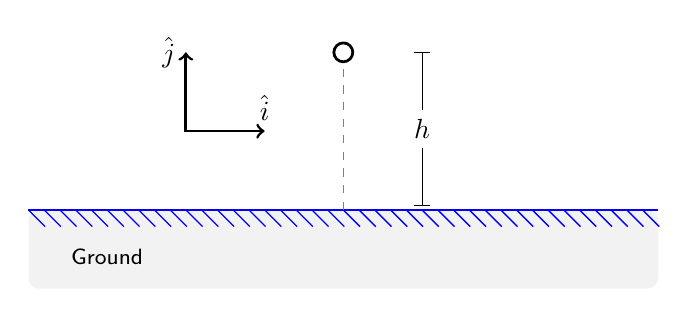
\begin{tikzpicture}[
    media/.style={font={\footnotesize\sffamily}},
    wave/.style={
        decorate,decoration={snake,post length=1.4mm,amplitude=2mm,
        segment length=2mm},thick},
    interface/.style={
        % The border decoration is a path replacing decorator. 
        % For the interface style we want to draw the original path.
        % The postaction option is therefore used to ensure that the
        % border decoration is drawn *after* the original path.
        postaction={draw,decorate,decoration={border,angle=-45,
                    amplitude=0.3cm,segment length=2mm}}},
    ]
    % Round rectangle
    \fill[gray!10,rounded corners] (-4,-1) rectangle (4,0);
    % Interface
    \draw[blue,line width=.5pt,interface](-4,0)--(4,0);

    % Vertical dashed line
    \draw[dashed,gray](0,0)--(0,2);
    
        % Vertical dashed line
    \draw[|-|](1,0.05)--(1,2) node[midway,fill=white]{$h$};
    
        % Coordinates system
    \draw[<->,line width=1pt] (-1,1) node[above]{$\hat{i}$}-|(-2,2) node[left]{$\hat{j}$};

    % Media names
    \path[media] (-3,-.6) node {Ground};

    % $x$ axis
    \filldraw[fill=white,line width=1pt](0,2)circle(.12cm);

\end{tikzpicture}
	\end{center}

	Align the coordinates such that $\hat{j}$ points upwards. We know that $\vec{a} = -g\hat{j}$. No motion in other directions. Problem is 1D!. 
	
	We know initially ($t=0$) that $y(0) = h \implies v_y(0) = 0$. Integrate twice: \[y(t) = h - \frac{1}{2}gt^2\]

\end{example}~

  \lecturemarker{3}{5 Oct}
\textbf{Recap:} 





\begin{example}[Projectile]
	
\begin{center}
	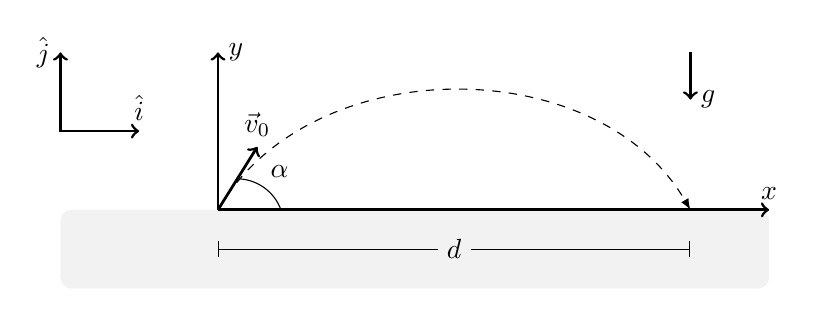
\begin{tikzpicture}[
    media/.style={font={\footnotesize\sffamily}},
    wave/.style={
        decorate,decoration={snake,post length=1.4mm,amplitude=2mm,
        segment length=2mm},thick},
    interface/.style={
        % The border decoration is a path replacing decorator. 
        % For the interface style we want to draw the original path.
        % The postaction option is therefore used to ensure that the
        % border decoration is drawn *after* the original path.
        postaction={draw,decorate,decoration={border,angle=-45,
                    amplitude=0.3cm,segment length=2mm}}},
    ]
    % Round rectangle
    \fill[gray!10,rounded corners] (-5,-1) rectangle (4,0);
    
    % Interface
    %\draw[blue,line width=.5pt,interface](-5,0)--(4,0);

    % Vertical dashed line
    %\draw[gray](-3,0)--(-3,2);
    
    % Coordinates system
    \draw[->,line width=1pt] (-3,0) --(4,0) node[above]{$x$};
    \draw[->,line width=1pt] (-3,0) --(-3,2) node[right]{$y$};
    
    % Coordinates system
    \draw[<->,line width=1pt] (-4,1) node[above]{$\hat{i}$}-|(-5,2) node[left]{$\hat{j}$};
    
        % Coordinates system
    \draw[->,line width=1pt] (3,2)--(3,1.4) node[right]{$g$};

        % Coordinates system
    \draw[->,line width=1pt] (-3,0)--(-2.5,0.8) node[above]{$\vec{v}_0$};


	 % Horizontal dashed line
    \draw[|-|](-3,-0.5)--(3,-0.5) node[midway, fill = gray!10]{$d$};


    % Media names
    %\path[media] (-3,-.6) node {Ground};
    
    
    \path (-3.2,0.3)++(11:1cm)node{$\alpha$};
    \draw[-](-2.2,0)arc(20:90:.6cm);

    
    % Interface pointer
    \draw[-latex,dashed](-3,0) to[out=60,in=120] (3,0);
    % To-paths are really useful for drawing curved lines. The above
    % to path is equal to:
    %
    % \draw[-latex,thick](3.2,0.5)node[right]{$\mathsf{S_{1,2}}$}
    %      ..controls +(180:.2cm) and +(up:0.25cm) .. (3,0);
    % Internally the to path is translated to a similar bezier curve,
    % but the to path syntax hides the complexity from the user. 

\end{tikzpicture}
	\end{center}
	
	In this coordinate system $\vec{a} = -g\hat{j}$. Choose that $t = 0$ when the object is released. Based on this: \[\vec{r}(0) = \vec{0},~\vec{v}(0) = \vec{v}_0 = v_0\cos\alpha\hat{i} + v_0\sin\alpha\hat{j}\]
	Integrate our acceleration to find $\vec{v}(t)$
	\[\begin{aligned}\vec{v}(t) &= \vec{v}(0) + \int_0^t -g\hat{j}\,dt' = \vec{v}_0 -gt\hat{j} \\ 
	&= v_0\cos\alpha\hat{i} + (v_0\sin\alpha -gt)\hat{j}
\end{aligned}
\]
	Integrate our velocity to find the position
	\[\begin{aligned}
\vec{r}(t) &= \vec{r}(0) + 	\int_0^t \vec{v}(t)\,dt' = \vec{0} + \int_0^t\vec{v}_0 -gt'\hat{j}\,dt'\\
&= \vec{v}_0t - \textstyle{\frac{1}{2}}t^2g\hat{j} = v_0t\cos\alpha\hat{i} + [v_0t\sin\alpha - \textstyle{\frac{1}{2}}t^2g]\hat{j}
\end{aligned}
\]

Maximise the \emph{range} using $\alpha$ as the control parameter. Finding the time $t_H$ when the object hits the ground. $y(t_H) = 0$ where $y = \vec{r}\cdot\hat{j}$. 
\[y = \vec{r}\cdot\hat{j}= v_0t_H\sin\alpha -\textstyle{\frac{1}{2}}t_H^2g = 0\]
Two values of $t_H$:
\[t_H = 0,~ t_H = \frac{2v_0\sin\alpha}{g}\]

To find the range:
\[x(t_H) = v_0\cos\alpha\left[\frac{2v_0\sin\alpha}{g}\right] = \frac{v_0^2}{g}\sin 2\alpha\]

For $0 \leq \alpha \leq \pi/2$, the range is maximum for $\alpha = \pi/4$.
\end{example}~

\begin{example}[Circular Motion]
\[\vec{r}(t) = R\sin(\Omega t)\hat{i} + R\cos(\Omega t)\hat{j}\]
where $R, \Omega$ are positive constraints. 

Distance from the origin 
\[r = |\vec{r}| = [R^2\sin^2\Omega t + R^2\cos^2\Omega t]^{1/2} = R\]

Path is a circle of radius $R$, centred at the origin. 


Differentiate $\vec{r}(t)$ to find $\vec{v}(t) = R\Omega \cos \Omega t\hat{i} - R\Omega \sin \Omega t \hat{j}$

Find the speed: $v = |\vec{v}| = R\Omega$, the speed is constant. 

Clockwise or anticlockwise? 

Direction of motion
\[\hat{v}= \vec{v}/v = \cos \Omega t\hat{i} - \sin\Omega t \hat{j}\]
At $t = 0$, $\hat{v}(0) = \hat{i}$, so it moves clockwise around the circle!

Interpretation of $\Omega$:

Introduce $\theta = -\Omega t + \pi/2$, $\frac{d\theta}{dt} - \Omega$. 

The parameter $\Omega$ is angular speed. Differentiate our $\vec{v}(t)$ we find
\[\begin{aligned}
\vec{a}(t) &= -R\Omega^2 \sin[\Omega t]\hat{i} - R\Omega^2\cos[\Omega t]\hat{j}\\
&= -\Omega^2 \vec{r}	
\end{aligned}
\]
Acceleration is pointing in towards the circle. 
\end{example}


  \lecturemarker{4}{5 Oct}


\subsektion{Vector Operations}  \lecturemarker{5}{5 Oct}

Already we have seen vector addition and subtraction are useful:

Addition: $\vec{r} = \vec{r}_C + \vec{r}_\Omega$

Subtraction: velociites relative to a moving observer $\vec{v}_{A,O} = \vec{v}_A - \vec{v}_O$


Vector Products: Vector products are also useful and do arise in describing mechanical phenomena: 

\begin{enumerate}
\item Scalar product (dot product)
\item 
\[\vec{A} \cdot \vec{B} = |\vec{A}||\vec{B}|\cos \theta\]

	
\end{enumerate}




\subsektion{Polar Coordinates}
\pagebreak


\subsektion{Intrinsic Coordinates}

\lecturemarker{7}{5 Oct}

Coordinates that are intrinsic to the path of our particle. We know the path!
\vspace*{120pt}

Distance travelled between $t$ and $t + \Delta t$
:
\[\Delta s = |\Delta \vec{r}| = \left|[x(t + \Delta t) - x(t)]\hat{i} + [y(t + \Delta t) - y(t)]\hat{j} + [z(t + \Delta t) - z(t)]\hat{k}\right|\]
For $\Delta t << 1$: 
\[x(t + \Delta t) = x(t) + \Delta t \frac{dx}{dt} + \cal{O}(\Delta t^2)\]
Doing the same for our other components:
\[\Delta s = \underbrace{\left|\frac{dx}{dt}\hat{i} + \frac{dy}{dt}\hat{j} + \frac{dz}{dt}\hat{k}\right|}_{\vec{v}}\Delta t + \cal{O}(\Delta t^2)\]

Thus,
\[\frac{\Delta s}{\Delta t} = v + \cal{O}(\Delta t)\]
Taking $\lim \Delta t \to 0$
\[\boxed{\frac{ds}{dt} = v = \dot{s} \implies s(t) = \int_0^t v(t')\,dt'}\]
Both $t$ and $s$ are ways of parametrizing our curve (path). Instead of writing $\vec{r}(t)$, we can write $\vec{r}(s)$. \\

\begin{definition} $s$ is what we call the \emph{arc length}. 

$\displaystyle{\vec{v} = \frac{d\vec{r}}{dt} = \frac{d\vec{r}}{ds}\frac{ds}{dt}}$. But $\displaystyle{\frac{ds}{dt} = v}$. So, $\displaystyle{\frac{d\vec{r}}{ds} = \hat{v}}$, the unit tangent at evert point $s$. Thus
\[\vec{v}(s) = \dot{s}\hat{v}\]

Also \[\begin{aligned}
	\vec{a} = \frac{d\vec{v}}{dt} = \frac{d}{dt}\left(\dot{s}~ \frac{d\vec{r}}{ds}\right) = \ddot{s}\frac{\d\vec{r}}{ds} + \dot{s}\frac{d}{dt}\left(\frac{d\vec{r}}{ds}\right) &= \ddot{s}\hat{v} + \dot{s}\frac{d^2\vec{r}}{ds^2}\frac{ds}{dt}
\end{aligned}
\]

So
\[\vec{a}(s) = \ddot{s}\hat{v} + \dot{s}^2\frac{d^2\vec{r}}{ds^2} = \ddot{s}\hat{v} + \kappa \dot{s}^2\hat{n}\]
Writing $\displaystyle{\frac{d^2\vec{r}}{ds^2} = \kappa \hat{n}}$, where $\displaystyle{\kappa =\left|\frac{d^2\vec{r}}{ds^2}\right| }$, $\hat{n} = \displaystyle{\frac{1}{\kappa}\frac{d^2\vec{r}}{ds^2}}$.
\end{definition}

It turns out that $\kappa$ is the curvature of the path. What about $\hat{n}$?

Recall: $|\hat{v}| = 1$. So $\frac{d}{ds}(\hat{v}\cdot\hat{v} = 1) \implies 2\hat{v}\cdot\frac{d\hat{v}}{ds} = 0 \implies 2\kappa(\hat{v}\cdot\hat{n}) = 0$

So, if $\kappa \neq 0$, then $\hat{v}\cdot \hat{n} = 0$. Thus $\hat{n}$ is the unit normal to the path.\\

Tangential component of the acceleration $a_t = \vec{a}\cdot\hat{v} = \ddot{s}$

Normal component of the acceleration $a_n = \vec{a}\cdot\hat{n} = \kappa \dot{s}^2$, where $\kappa \approx 1/R$
\vspace*{100pt}

Key things to note: $\hat{v}, \hat{n}, \kappa$ depend only on the path. Knowing $\vec{r}(s)$, we can find these 	quantities. 

$\dot{s}$ and $\ddot{s}$ depend on how the particle is moving along the path.\\


\begin{example}[Circular Motion]~\\

\textbf{Cartesian:}
$\vec{r}(t) = R\sin(\omega t)\hat{i} + R\cos(\omega t)\hat{j}$.
Differentiating finds $\vec{v}(t)$ and $\vec{a}(t)$.\\

\textbf{Polars:} 
$r = R$ and $\theta = \frac{\pi}{2} \omega t \implies \dot{r} = \ddot{r} = 0$ and $ \dot{\theta} = -\omega,~\ddot{\theta} = 0$. So 

\[\begin{aligned}
	\vec{r} &= R\hat{r}\\
 \vec{v} &= \dot{r}\hat{r} + r\dot{\theta}\hat{\theta} = -R\omega\hat{\theta}\\
\vec{a} &= (\ddot{r} - r\dot{\theta}^2)\hat{r} + (2\dot{r}\dot{\theta} + r\ddot{\theta})\hat{\theta} = -R\omega^2\hat{r}
\end{aligned}
\]~

\textbf{Intrinsic:} ($s(0) = 0$) The speed is given by $v = R\omega = \dot{s} \implies \ddot{s} = 0$. Integrate to find $s$
\[s = R\omega t \implies t= \frac{s}{R\omega}\]
Substitute this into our expression for $\vec{r}(t)$
\[\vec{r}(s) = R\sin(s/R)\hat{i} + R\cos(s/R)\hat{j}\]

$\implies \hat{v} = \dfrac{d\vec{r}}{ds} = \cos(s/R)\hat{i} - \sin(s/R)\hat{j}$,
$~~\dfrac{d^2\vec{r}}{ds^2} = -\dfrac{1}{R}[\sin(s/R)\hat{i} + \cos(s/R)\hat{j}]$

$\implies \kappa = \left|\dfrac{d^2\vec{r}}{ds^2} \right| = \dfrac{1}{R}$, $\hat{n} = -\sin(s/R)\hat{i} - \cos(s/R)\hat{j}$

\[\begin{aligned}
\vec{v}(s) &= R\omega \hat{v}\\
\vec{a}(s) &= \ddot{s}\hat{v} + \kappa \dot{s}^2\hat{n} = \frac{1}{R}(R\omega)^2\hat{n} = R\omega^2\hat{n}
\end{aligned}
\]
\end{example}


\begin{example}[Helical Path]\lecturemarker{8}{5 Oct}
	\[\vec{r}(s) = b\cos(ks)\hat{i} + b\sin(ks)\hat{j} + s\sqrt{1-b^2k^2}\hat{k}\]
	
	Tangent:
	\[\vec{v} = \frac{d\vec{r}}{ds} = -bk\sin(ks)\hat{i} + bk\cos(ks)\hat{j} + \sqrt{1-b^2k^2}\hat{k}\]~
	
	Curvature and Normal:
	\[\frac{d^2\vec{r}}{ds^2} = -bk^2\cos(ks)\hat{i} -bk^2 \sin(ks)\hat{j}\]
	\[\kappa =\left|\frac{d^2\vec{r}}{ds^2}\right| = bk^2,~ \hat{n} =  -\cos(ks)\hat{i} -\sin(ks)\hat{j}\]
	
Take $s = ct$ ($c >0$) $ \implies \dot{s} =c,~ \ddot{s} = 0$. Thus
\[\vec{v} = c\hat{v},~\vec{a} = c^2bk^2\hat{n}\]	
\end{example}

Take the case where our path lies in the $xy-$plane and we know $y(x)$
\vspace*{100pt}

Then $ds^2 = dx^2 + dy^2$. Since $dy = \frac{dy}{dx}dx \implies ds^2 = (1 + (\frac{dy}{dx})^2 )dx^2$
\[\implies \frac{ds}{dx} = \sqrt{1 + y'^2}\]
\[s(x) = \int_{x_0}^x (1 + y'^2)^{1/2}dx\]

Highlights that $s$ just depends on the path. 


Position $\vec{r}(x) = x\hat{i} + y(x)\hat{j}$

Tangent to the path
\[\hat{v} = \frac{d\vec{r}}{ds} = \frac{d\vec{r}}{dx}\frac{dx}{ds} = \frac{d\vec{r}}{dx}\left(\frac{ds}{dx}\right)^{-1}\]
\[\frac{d\vec{r}}{dx} = \hat{i} + y'\hat{j},~~\left(\frac{ds}{dx}\right)^{-1} = [1 + y'^2]^{-1/2}\]
\[\implies \hat{v} = [1+y'2]^{-1/2}[\hat{i} + y'\hat{j}]\]

Curvature and Normal
\[\frac{d^2\vec{r}}{ds^2} = \frac{d}{dx}\left(\frac{d\vec{r}}{ds}\right)\left(\frac{ds}{dx}\right)^{-1} = \left(\frac{d}{dx}\left(\frac{d\vec{r}}{ds}\right)\frac{dx}{ds}\right)\]
\[\frac{d}{dx}\frac{d\vec{r}}{ds} = \frac{d\hat{v}}{dx} = -\frac{1}{2}[1+y'^2]^{-3/2} \times (2y'y'')\times [\hat{i} + y'\hat{j}] + [1 + y'^2]^{-1/2}y''\hat{j}\]~


\begin{example}
$y = x^2,~y' = 2x,~ y'' = 2$

\[\frac{ds}{dx} = [1 + y'^2]^{1/2}\]	
\end{example}








